\chapter{Background}
\label{background}

\section{Blockchain}

A blockchain is a decentralized, distributed ledger technology that enables secure, transparent, and tamper-resistant storage of digital records across a network of participants. It consists of a series of blocks, each containing a list of transactions, which are cryptographically linked and secured using cryptographic algorithms. This structure allows for enhanced security and data integrity, as altering the information in one block would require most network participants' consensus and modifying all subsequent blocks.

Although initially developed for supporting cryptocurrencies like Bitcoin, blockchain technology has evolved to accommodate various applications across many industries, such as finance, supply chain, healthcare, and more \cite{Xu2019} \cite{ibm-blockchain}. Ethereum has emerged as a leading platform for developing and deploying smart contracts among the different blockchain platforms.

\subsection{Etherum Blockchain}

The Ethereum blockchain, launched in 2015 by Vitalik Buterin and his team, was designed to facilitate the creation, management, and execution of decentralized applications (DApps) and smart contracts. Unlike Bitcoin, which is primarily used for transferring digital currency, Ethereum provides a decentralized virtual machine—the Ethereum Virtual Machine (EVM)—which can execute arbitrary Turing-complete code on the blockchain \cite{hildenbrandt2017kevm}. This feature allows developers to build and deploy more complex and versatile applications on the Ethereum platform.

Smart contracts are self-executing contracts with the terms of the agreement directly written into code. They automatically execute and enforce the contract's terms when predefined conditions are met without the need for intermediaries. This enables secure, decentralized, and automated transactions on the blockchain, leading to increased efficiency and reduced transaction costs. Ethereum's native cryptocurrency, Ether (ETH), is used to pay for the computational resources and transaction fees required to execute smart contracts on the network. A pertinent fact in this research is that once a smart contract is deployed on the Ethereum blockchain, it cannot be modified or removed. This immutability makes smart contracts a highly attractive target for attackers, as they can potentially cause significant financial losses and damage the organization's reputation. For this reason, smart contracts must be developed and deployed securely.

\subsection{The Solidity Language}

Solidity is a high-level, statically-typed, contract-oriented programming language specifically designed for writing smart contracts on the Ethereum blockchain. Created by Dr. Gavin Wood, Christian Reitwiessner, and their team at Ethereum, Solidity is influenced by other programming languages such as JavaScript, Python, and C++, and is designed to target the Ethereum Virtual Machine (EVM). The EVM executes the compiled bytecode of the smart contracts, which is generated from the Solidity source code.

\subsubsection{Syntax and Structure}

Solidity syntax is similar to JavaScript and employs a curly-bracket ({}) notation for defining code blocks. A Solidity smart contract typically starts with a \textit{pragma} directive, which specifies the version of the Solidity compiler required for the source code. This is followed by the contract definition, which includes the contract's state variables, functions, events, and access modifiers.

\begin{verbatim}
pragma solidity ^0.8.0;

contract SimpleStorage {
    uint256 private storedData;


    function set(uint256 x) public {
        storedData = x;
    }

    function get() public view returns (uint256) {
        return storedData;
    }

}
\end{verbatim}

The example above demonstrates a simple Solidity contract, \textit{SimpleStorage}, which allows users to store and retrieve an unsigned 256-bit integer value. The contract consists of a private state variable, \textit{storedData}, and two public functions, \textit{set()} and \textit{get()}.

\subsubsection{Data Types and Variables}

Solidity supports various data types, including value types (such as integers, booleans, and addresses) and reference types (such as arrays, mappings, and structs). Additionally, Solidity allows for the declaration of user-defined types, such as enums and structs, to create more complex data structures.

\subsubsection{Functions and Modifiers}

Functions in Solidity are similar to functions in other programming languages, defining a reusable block of code that performs a specific task. Functions can be declared as public, private, external, or internal, which determines their visibility and accessibility within the contract and by other contracts. Functions can also be marked as \textit{view} or \textit{pure}, indicating that they do not modify the contract's state and only read or compute data, respectively.

Modifiers can be used to alter the behavior of functions by appending or prepending additional code to the function's body. They are often used to enforce access control, by requiring certain conditions to be met before the function can be executed, such as requiring the sender to be the contract owner.

\subsubsection{Events and Inheritance}

Events are used in Solidity to emit logs that can be monitored by the contract's users, allowing them to be notified of specific occurrences or state changes within the contract. This is particularly useful for creating event-driven applications and tracking transactions on the Ethereum blockchain.

Solidity also supports inheritance, allowing contracts to inherit properties and methods from other contracts. This enables code reuse and modularity, facilitating the development of complex and robust smart contracts.

By understanding the fundamentals of Solidity and its features, developers can create secure and efficient smart contracts on the Ethereum platform. The background knowledge on Solidity provided in this subsection serves as a foundation for the subsequent analysis of smart contract vulnerabilities and the evaluation of ESBMC in this study.

\section{Smart Contract Vulnerabilities}

Smart contract vulnerabilities are security flaws, weaknesses, or design errors in implementing smart contracts, which can lead to unintended behavior or exploitation by malicious actors. Due to the decentralized and transparent nature of blockchain technology and the irreversible nature of transactions on the blockchain, addressing and mitigating these vulnerabilities is paramount for ensuring the security, trustworthiness, and stability of blockchain ecosystems.

Several high-profile incidents, such as the DAO hack in 2016 and the Parity wallet multi-signature vulnerability in 2017 \cite{smartcon-vulnerabilities}, have demonstrated the significant financial and reputational risks associated with smart contract vulnerabilities. These incidents have spurred an increased interest in the research and development of tools and techniques for identifying and mitigating vulnerabilities in smart contracts.

As Ethereum is one of the most widely-used platforms for developing and deploying smart contracts, understanding and addressing vulnerabilities in Ethereum-based smart contracts is crucial for the broader blockchain community. 

\subsection{Smart Contract Weakness Classification (SWC) Registry}

The Smart Contract Weakness Classification (SWC) Registry \cite{swc} is a comprehensive and well-maintained collection of known vulnerabilities and weaknesses in smart contracts. This registry enables developers, security researchers, and auditors to communicate effectively about smart contract security issues and to foster collaboration in addressing them. The MythX team established the SWC Registry to provide a common language and taxonomy for identifying and categorizing smart contract vulnerabilities.

By classifying smart contract weaknesses into distinct categories, the SWC Registry allows for a better understanding and awareness of these vulnerabilities, facilitating more secure coding practices and robust smart contract development. Each vulnerability listed in the SWC Registry is assigned a unique SWC identifier and includes detailed information, such as its description, impact, potential mitigation, and examples.

Some common vulnerability categories in the SWC Registry are:

\begin{itemize}
\item Reentrancy (SWC-107)
\item Arithmetic Issues (e.g., Integer Overflow and Underflow) (SWC-101)
\item Insecure DelegateCall Implementation (SWC-112)
\item Authorization through tx.origin (SWC-115)
\end{itemize}

As part of this project, the SWC Registry is a valuable resource for understanding smart contract vulnerabilities, their consequences, and mitigation techniques. By referring to the SWC Registry, the benchmark suite of vulnerable smart contracts is developed to cover a wide range of security weaknesses, ensuring a comprehensive evaluation of ESBMC's effectiveness in detecting and mitigating these vulnerabilities.

Moreover, using the SWC Registry's taxonomy and classification system, this study aims to present a structured and systematic analysis of ESBMC's performance, making it easier for other researchers and developers to compare and contrast the results with those of alternative model-checking tools or verification techniques. This, in turn, will contribute to the overall improvement and advancement of smart contract security research and the development of more secure and reliable blockchain ecosystems.

\begin{table}
\begin{center}
    \begin{tabular}{ |c|c|c| } 
     \hline
     \textbf{SWC ID} & \textbf{Vulnerability Title} & \textbf{Section} \\
        SWC-100 & Function Default Visibility & \ref{sec:default_visibility}\\
        SWC-101 & Integer Overflow and Underflow & \ref{sec:integer_overflow} \\
        SWC-102 & Outdated Compiler Version & \ref{sec:outdated_compiler} \\
        SWC-103 & Floating Pragma & \ref{sec:floating_pragma} \\
        SWC-104 & Unchecked Call Return Value & \ref{sec:unchecked_call_return_value} \\
        SWC-105 & Unprotected Ether Withdrawal & \ref{sec:unprotected_ether_withdrawal} \\
        SWC-106 & Unprotected Self-Destruct & \ref{sec:unprotected_self_destruct} \\
        SWC-107 & Reentrancy & \ref{sec:reentrancy} \\
        SWC-108 & State Variable Default Visibility & \ref{sec:state_variable_default_visibility} \\
        SWC-109 & Unitialized Storage Pointer & \ref{sec:uninitialized_storage_pointer} \\
        SWC-110 & Assert Violation & \ref{sec:assert_violation} \\
        SWC-111 & Use of Deprecated Solidity Functions & \ref{sec:use_of_deprecated_solidity_functions} \\
        SWC-112 & DelegateCall to Untrusted Contract & \ref{sec:delegatecall_to_untrusted_callee} \\
        SWC-113 & DoS with Failed Call & \ref{sec:dos_with_failed_call} \\
        SWC-114 & Transaction Order Dependence & \ref{sec:other_vulnerabilities} \\
        SWC-115 & tx.origin Authentication & \ref{sec:authorization_through_tx.origin} \\
        SWC-116 & Block values as a Proxy for Time & \ref{sec:block_values_as_a_proxy_for_time} \\
        SWC-117 & Signature Malleability & \ref{sec:other_vulnerabilities} \\
        SWC-118 & Incorrect Constructor Name & \ref{sec:incorrect_constructor_name} \\
        SWC-119 & Shadowing State Variables & \ref{sec:shadowing_state_variables} \\
        SWC-120 & Weak Sources of Randomness & \ref{sec:weak_sources_of_randomness_from_chain_attributes} \\
        SWC-121 & Missing Protection against Signature Replay Attacks & \ref{sec:missing_protection_against_signature_replay_attacks} \\
        SWC-122 & Lack of Proper Signature Verification & \ref{sec:lack_of_proper_signature_verification} \\
        SWC-123 & Requirement Violation & \ref{sec:requirement_violation} \\
        SWC-124 & Write to Arbitrary Storage Location & \ref{sec:write_to_arbitrary_storage_location} \\
        SWC-125 & Incorrect Inheritance Order & \ref{sec:other_vulnerabilities} \\
        SWC-126 & Insufficient Gas Griefing & \ref{sec:insufficient_gas_griefing} \\
        SWC-127 & Arbitrary Jump with Function Type Variable & \ref{sec:other_vulnerabilities} \\
        SWC-128 & DoS With Block Gas Limit & \ref{sec:other_vulnerabilities} \\
        SWC-129 & Typographical Error & \ref{sec:typographical_error} \\
        SWC-130 & Right-To-Left-Override control character (U+202E) & \ref{sec:other_vulnerabilities} \\
        SWC-131 & Presence of unused variables & \ref{sec:presence_of_unused_variables} \\
        SWC-132 & Unexpected Ether balance & \ref{sec:unexpected_ether_balance} \\
        SWC-133 & Hash Collisions With Multiple Variable Length Arguments & \ref{sec:hash_collisions_with_multiple_variable_length_arguments} \\
        SWC-134 & Message call with hardcoded gas amount & \ref{sec:message_call_with_hardcoded_gas_amount} \\
        SWC-135 & Code with No Effect & \ref{sec:other_vulnerabilities} \\
        SWC-136 & Unencrypted Private Data On-Chain & \ref{sec:unencrypted_private_data_on_chain} \\
     \hline
    \end{tabular}
\label{tab:swc}
\end{center}
\caption{SWC Vulnerabilities as Identified on the SWC Registry \cite{swc}}
\end{table}
\section{ESBMC: Efficient SMT-based Bounded Model Checker}

The Efficient SMT-based Bounded Model Checker (ESBMC) is a state-of-the-art software verification tool designed to check the correctness and reliability of programs written in C, C++, and Solidity languages. ESBMC employs Satisfiability Modulo Theories (SMT) solvers to perform bounded model checking, a formal verification technique that explores the state space of a program to detect and analyze potential errors, bugs, or security vulnerabilities within a predefined number of execution steps.

\subsection{ESBMC's Capabilities}

ESBMC is equipped with several advanced features and capabilities that make it a powerful and versatile tool for software verification, particularly in the context of smart contract security. Some of the key capabilities of ESBMC include:

\begin{itemize}

\item \textbf{Bounded Model Checking}: ESBMC uses bounded model checking to explore the state space of a program within a specified depth limit. This technique allows for efficient and scalable verification of complex programs, making ESBMC suitable for analyzing real-world smart contracts with complex logic and interactions.

\item \textbf{SMT Solvers}: ESBMC employs various SMT solvers, such as Z3, CVC4, and Collector, facilitating efficient decision-making and constraint-solving during the verification process. The integration of these solvers enables ESBMC to effectively analyze complex mathematical operations, data structures, and program behaviors.

\item \textbf{Assertion Checking and Invariant Generation}: ESBMC can automatically check user-defined assertions and generate invariants for loops and other program constructs. This capability enables the detection of potential errors or vulnerabilities that could violate a smart contract's intended behavior or safety properties.

\item \textbf{Concurrency Support}: ESBMC provides support for verifying concurrent programs, allowing for the detection and analysis of potential race conditions, deadlocks, and other concurrency-related issues in smart contracts.

\end{itemize}

With these capabilities, ESBMC has the potential to become an effective tool for detecting and mitigating vulnerabilities in Ethereum-based smart contracts. In this study, we aim to evaluate ESBMC's performance and effectiveness in identifying and addressing vulnerabilities within a benchmark suite of intentionally vulnerable smart contracts, ultimately contributing to developing more secure and reliable verification techniques for smart contract security.

\subsection{ESBMC and Solidity}

The current implementation of ESBMC's solidity frontend is a developing area, defined as an "early prototype" in the ESBMC documentation \cite{esbmc_doc}. ESBMC does not support the full Solidity language at the time of writing. Currently supported is the ability to check individual functions for many common vulnerabilities. However, reviewing whole smart contracts is not fully supported, nor are many key elements of the Object Oriented Programming (OOP) paradigm in Solidity. These unfinished features will become limiting for many of the vulnerabilities in the SWC Registry \cite{swc}, as many of them are related to the OOP paradigm or the functionality of a smart contract.

\subsection{ESBMC's Verification Process}

ESBMC takes an input of a solidity smart contract. It then performs a series of steps to verify the smart contract. These steps are shown in Figure \ref{fig:ESBMC_process}. The first step is to parse the smart contract into an intermediate representation (IR); in this case, we use an AST (Abstract Syntax Tree). The AST is then converted into a GOTO program, processed by the symbolic execution engine (SymEx), giving us a static single assignment (SSA) form. The SSA form is then passed to the SMT Solvers (for example, Bitwuzla, Boolector, CVC4, or Yices), which check for errors. The SMT solver will return a counterexample if it finds an error, which is then used to generate a test case. The test case is then used to generate a trace, which is then used to generate a counterexample. The counterexample is then used to generate a bug report, which is then outputted to the user \cite{song2022esbmc}. Further details on SMT-based solving can be found in \textit{SMT-based bounded model checking for embedded ANSI-C software} \cite{cordeiro2011smt}, and it is beyond the scope of this project.


\begin{figure}[h]
\centering
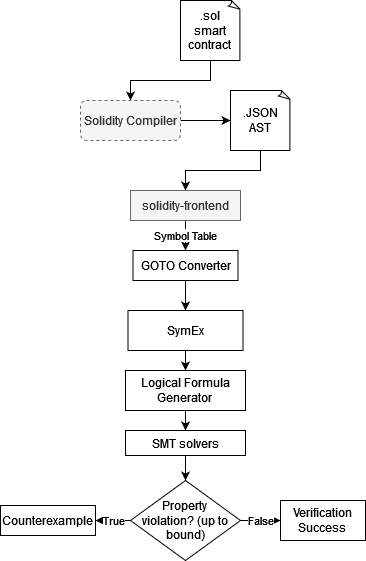
\includegraphics{ESBMC_process.png}
\caption{ESBMC's Verification Process \cite{song2022esbmc}}
\label{fig:ESBMC_process}
\end{figure}